\documentclass{standalone}
\usepackage{tikz}
\usepackage{pgfplots}
\usetikzlibrary{arrows.meta}

\begin{document}

\resizebox{8cm}{8cm}{%
    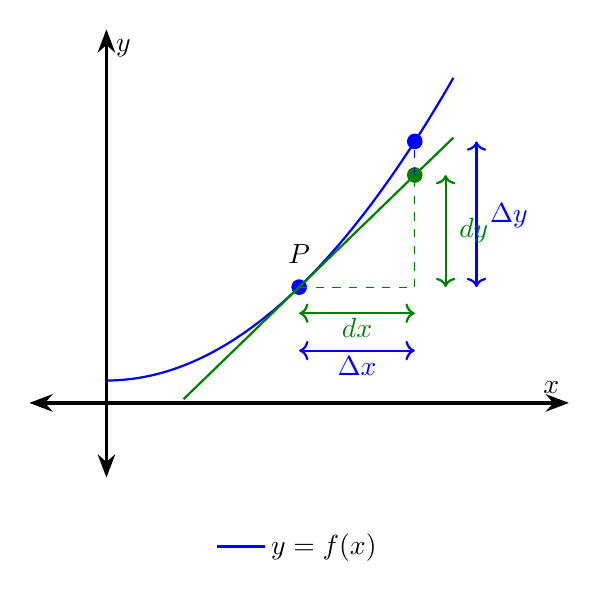
\begin{tikzpicture}
    \begin{axis}[
        title={},
        axis lines=middle,
        axis line style={Stealth-Stealth,very thick},
        xlabel=$x$,
        ylabel={$y$},
        xmin=-2,xmax=12,ymin=-1,ymax=5,
        xtick=\empty,
        ytick=\empty,
        % grid=major,
        % grid style={thin,densely dotted,black!20},
        % Numbers on axes
        % xtick={-8,-7,-6,-5,-4,-3,-2,-1,0,1,2,3,4,5,6,7,8},
        % xtick={-8,-7,-6,-5,-4,-3,-2,-1,0,1,2,3,4,5,6,7,8},
        % Legend
        legend style={
            at={(0.5,-0.1)}, % Position at the center bottom
            anchor=north, % Anchor the legend at the top
            cells={anchor=west}, % Align the legend entries to the left
            draw=none % no box around the legend
        }
    ]

    % -------------------------------------------------------
    % Plot the curve y = f(x) - BLUE
    \addplot[
        domain=0:9,
        samples=200,
        color=blue,
        thick
        ]
        {0.05*x^2 + 0.3};
    \addlegendentry{$y = f(x)$}

    % Mark point P at (5, 1.55)
    \node[circle, fill=blue, inner sep=2pt, label={[label distance=2pt]above:$P$}] at (axis cs:5,1.55) {};
    % Mark point on curve at x + dx (the Δy endpoint)
    \node[circle, fill=blue, inner sep=2pt] at (axis cs:8,3.5) {};

    % Δx bracket: further below
    \draw[<->, thick, blue] (axis cs:5,0.7) -- (axis cs:8,0.7);
    \node[blue] at (axis cs:6.5,0.5) {$\Delta x$};
    % Δy bracket: between Rail 1 (bottom) and Rail 3 (top), further right
    \draw[<->, thick, blue] (axis cs:9.6,1.55) -- (axis cs:9.6,3.5);
    \node[blue, right] at (axis cs:9.7,2.5) {$\Delta y$};

    % -------------------------------------------------------
    % Plot the tangent line at P - GREEN
    \addplot[
        domain=2:9,
        samples=2,
        color=green!50!black,
        thick
        ]
        {0.5*x - 0.95};

    % Mark point on tangent at x + dx (the dy endpoint)
    \node[circle, fill=green!50!black, inner sep=2pt] at (axis cs:8,3.05) {};

    % Horizontal dashed line for Δx (from P over to under the curve point)
    \draw[dashed, green!50!black] (axis cs:5,1.55) -- (axis cs:8,1.55);
    % Vertical dashed line — bottom half (green): represents dy
    \draw[dashed, green!50!black] (axis cs:8,1.55) -- (axis cs:8,3.05);
    % Vertical dashed line — top half (blue): the gap between dy and Δy
    \draw[dashed, blue] (axis cs:8,3.05) -- (axis cs:8,3.5);

    % dx bracket: closer to P's level
    \draw[<->, thick, green!50!black] (axis cs:5,1.2) -- (axis cs:8,1.2);
    \node[green!50!black] at (axis cs:6.5,1.0) {$dx$};
    % dy bracket: between Rail 1 (bottom) and Rail 2 (middle), to the right of the rails
    \draw[<->, thick, green!50!black] (axis cs:8.8,1.55) -- (axis cs:8.8,3.05);
    \node[green!50!black, right] at (axis cs:8.9,2.3) {$dy$};

    \end{axis}
    \end{tikzpicture}
}

\end{document}